\documentclass [a4 paper,11pt]{report}
\usepackage [french]{babel}
\usepackage [utf8]{inputenc}
\usepackage{graphicx}
\usepackage[T1]{fontenc}
\usepackage{textcomp}
\usepackage{listingsutf8}
\usepackage{xcolor}
\usepackage{textcomp}
\usepackage{float}
\usepackage{hyperref}
\usepackage{fancyhdr}

\lstset{
inputencoding=utf8/latin1,
belowcaptionskip=1\baselineskip,
inputencoding=utf8/latin1,
breaklines=true,
frame=L,
xleftmargin=\parindent,
language=c++,
showstringspaces=false,
basicstyle=\footnotesize\ttfamily,
keywordstyle=\bfseries\color{purple!40!black},
commentstyle=\itshape\color{green!40!black},
identifierstyle=\color{black},
stringstyle=\color{blue},
}

\title {Compte rendu TP traiment d'images}
\author {
\bsc{LE PHILIPPE} Noé\\
}
\date{\today}

\begin{document}
\makeatletter
 
\maketitle
\section*{Algorithmes}

\subsection*{Seuillage de l'image}
\begin{lstlisting}
/**
La valeur est mise a 0 si elle est inferieure au seuil et mise
au maximum d'un short si elle est superieure
*/
void RawReader::seuil(unsigned short s) {
  for (int i = 0; i < sizeX; ++i) {
    for (int j = 0; j < sizeY; ++j) {
      for (int k = 0; k < sizeZ; ++k) {
        if(getValue(i, j, k) < s) {
          setValue(i, j, k, 0);
        } else {
          setValue(i, j, k, pow(2, 16) - 1);
        }
      }
    }
  }
}
\end{lstlisting}
\newpage
\subsection*{Marching Cubes}
\begin{lstlisting}
/**
Parcours de tous les voxels adjacents et affichage des triangles correspondants
seulement s'ils sont superieurs au seuil.
*/
void RawReader::marchingCubes(double vWidth, double vHeight, double vDepth, unsigned short threshold) {
  std::cout << "solid name" << std::endl;
  for (int i = 1; i < sizeX - 1; ++i) {
    for (int j = 1; j < sizeY - 1; ++j) {
      for (int k = 1; k < sizeZ - 1; ++k) {

        if(getValue(i, j, k) > threshold) {

          if(getValue(i + 1, j, k) < threshold) {
            Vector orig((i + 1) * vWidth, j * vHeight, k * vDepth);
            Vector v1(0, 0, vDepth);
            Vector v2(0, vHeight, vDepth);
            Vector v3(0, vHeight, 0);
            Triangle t1(&orig, &v1, &v2, &v3);
            std::cout << t1.toString() << std::endl;
          }

          if(getValue(i - 1, j, k) < threshold) {
            Vector orig((i - 1) * vWidth, j * vHeight, k * vDepth);
            Vector v1(0, 0, vDepth);
            Vector v2(0, vHeight, vDepth);
            Vector v3(0, vHeight, 0);
            Triangle t1(&orig, &v1, &v2, &v3);
            std::cout << t1.toString() << std::endl;
          }

          if(getValue(i, j + 1, k) < threshold) {
            Vector orig(i * vWidth, (j + 1) * vHeight, k * vDepth);
            Vector v1(0, 0, vDepth);
            Vector v2(vWidth, 0, vDepth);
            Vector v3(vWidth, 0, 0);
            Triangle t1(&orig, &v1, &v2, &v3);
            std::cout << t1.toString() << std::endl;
          }
          if(getValue(i, j - 1, k) < threshold) {
            Vector orig(i * vWidth, (j - 1) * vHeight, k * vDepth);
            Vector v1(0, 0, vDepth);
            Vector v2(vWidth, 0, vDepth);
            Vector v3(vWidth, 0, 0);
            Triangle t1(&orig, &v1, &v2, &v3);
            std::cout << t1.toString() << std::endl;
          }
          if(getValue(i, j, k + 1) < threshold) {
            Vector orig(i * vWidth, j * vHeight, (k + 1) * vDepth);
            Vector v1(0, vHeight, 0);
            Vector v2(0, vHeight, 0);
            Vector v3(vWidth, 0, 0);
            Triangle t1(&orig, &v1, &v2, &v3);
            std::cout << t1.toString() << std::endl;
          }
          if(getValue(i, j, k - 1) < threshold) {
            Vector orig(i * vWidth, j * vHeight, (k - 1) * vDepth);
            Vector v1(0, vHeight, 0);
            Vector v2(vWidth, 0, 0);
            Vector v3(vWidth, vHeight, 0);
            Triangle t1(&orig, &v1, &v2, &v3);
            std::cout << t1.toString() << std::endl;
          }
        }
      }
    }
  }
  std::cout << "endsolid name" << std::endl;
}
\end{lstlisting}

\subsection*{Classe Triangle}
\begin{lstlisting}
class Triangle {
  /**
    un triangle est compose de 3 points representes par des vecteurs
  */
public:
  Vector *v1;
  Vector *v2;
  Vector *v3;

  /**
    les vecteurs sont construits à partir d'un point d'origine : le sommet du voxel
  */
  Triangle(Vector* orig, Vector* x, Vector* y, Vector* z) {
    this->v1 = new Vector(orig->x, orig->y, orig->z); v1->add(x->x, x->y, x->z);
    this->v2 = new Vector(orig->x, orig->y, orig->z); v2->add(y->x, y->y, y->z);
    this->v3 = new Vector(orig->x, orig->y, orig->z); v3->add(z->x, z->y, z->z);
  }

  /**
  affichage des coordonnees de chaque extremite du triangle
  */
  std::string toString() {
    std::string s = "facet normal 0 0 0";

    s += "\nouter loop\n";
    s += "vertex " + v1->toString() + "\n";
    s += "vertex " + v2->toString() + "\n";
    s += "vertex " + v3->toString() + "\n";
    s += "endloop\nendfacet";
    
    return s;
  }
};
\end{lstlisting}

\section*{Classe Vector}
\begin{lstlisting}
class Vector {
public:
  double x;
  double y;
  double z;

  Vector(double x, double y, double z) {
    this->x = x;
    this->y = y;
    this->z = z;
  }

  void add(double x, double y, double z) {
    this->x += x;
    this->y += y;
    this->z += z;
  }

  std::string toString() {
    string s = "";
    s += std::to_string(x) + " ";
    s += std::to_string(y) + " ";
    s += std::to_string(z);
    return s;
  }

};
\end{lstlisting}
\newpage
\section*{Sortie de l'application}
Tous les triangles ne sont pas affichés pour des raisons de performance et de taille des fichiers

\begin{figure}[h!]
\noindent\makebox[\textwidth]{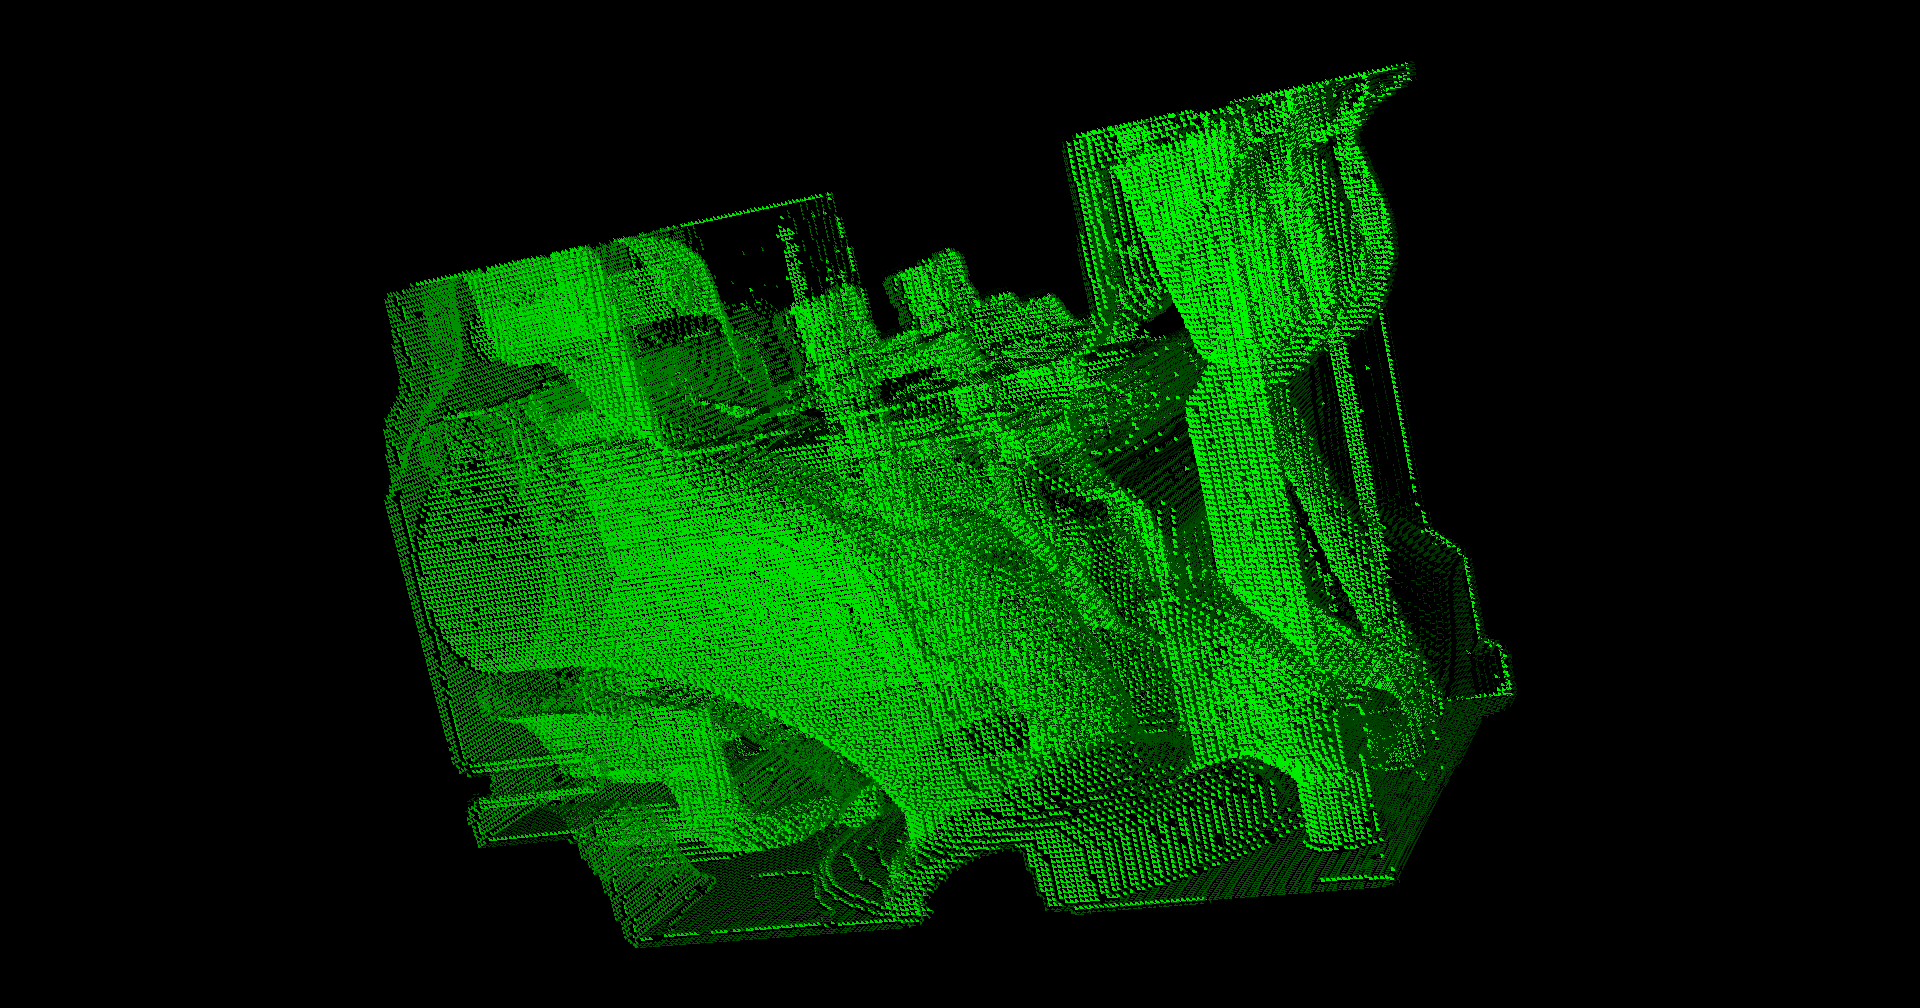
\includegraphics[width=200pt]{engine_100.png}}
\caption{Engine - seuil de 100}
\end{figure}

\begin{figure}[h!]
\noindent\makebox[\textwidth]{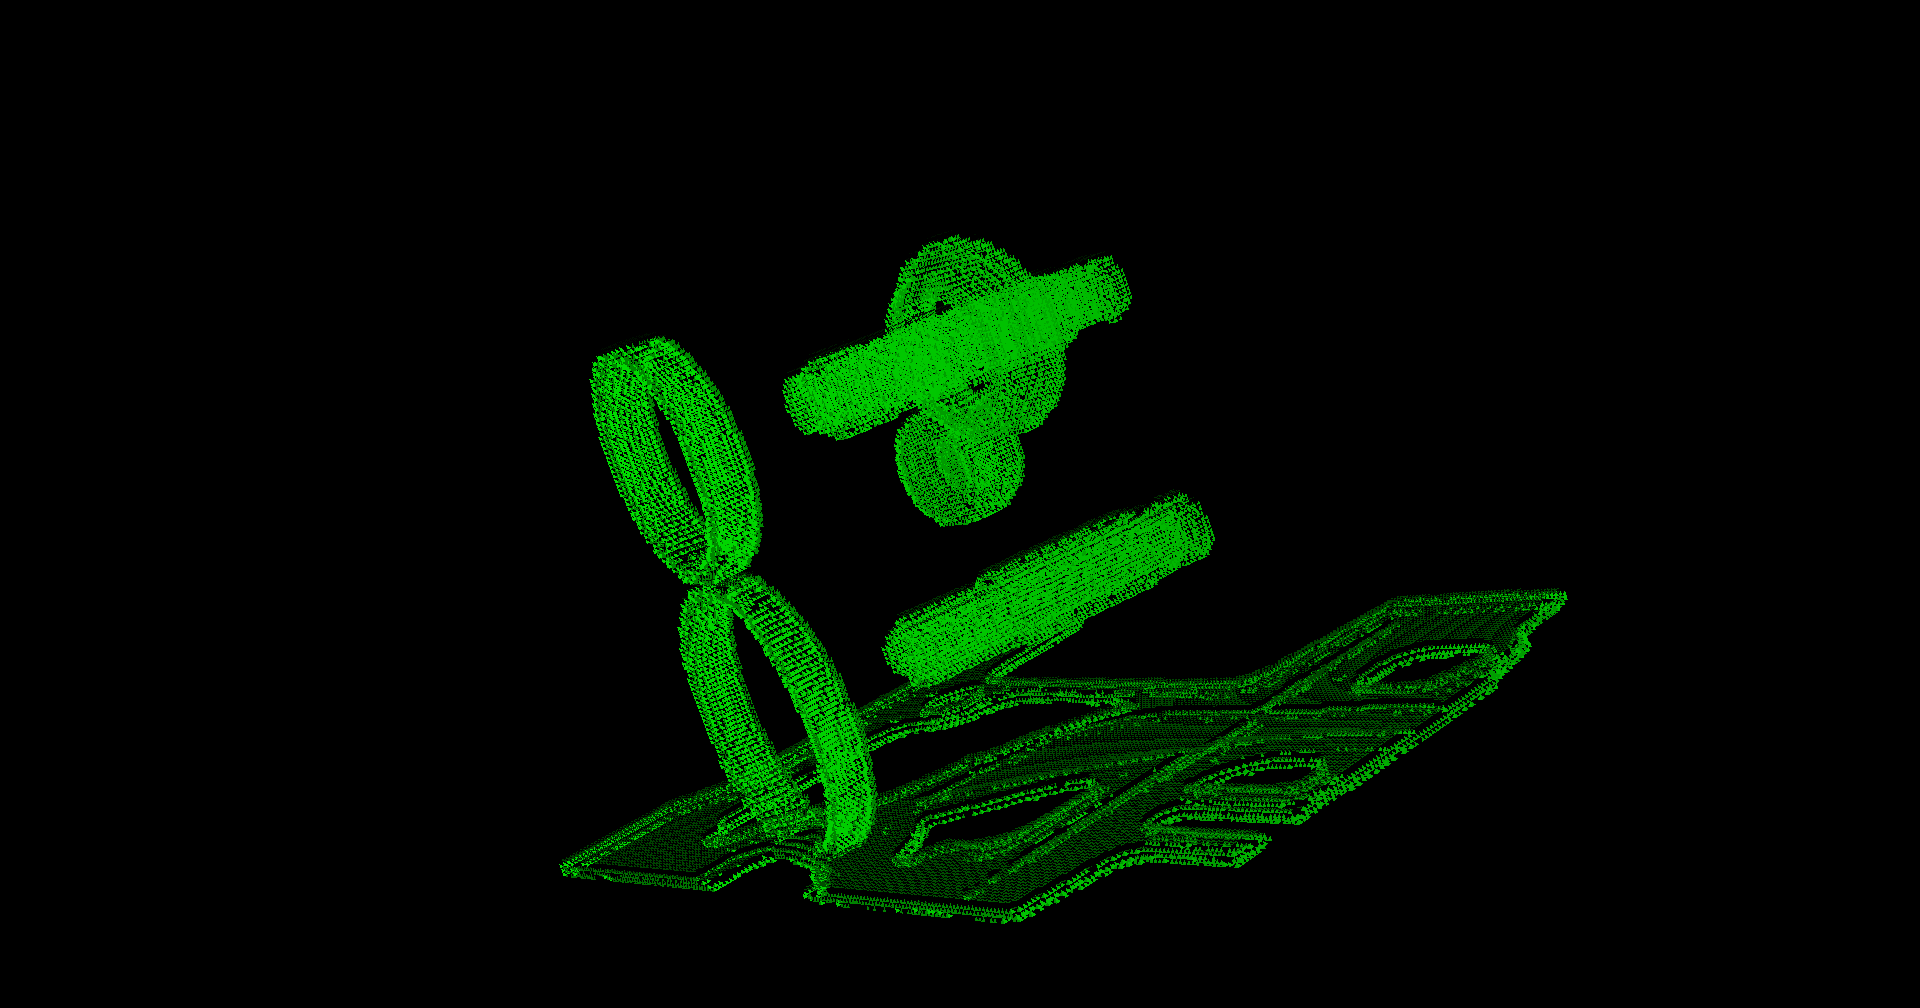
\includegraphics[width=200pt]{engine_200.png}}
\caption{Engine - seuil de 200}
\end{figure}

\begin{figure}[h!]
\noindent\makebox[\textwidth]{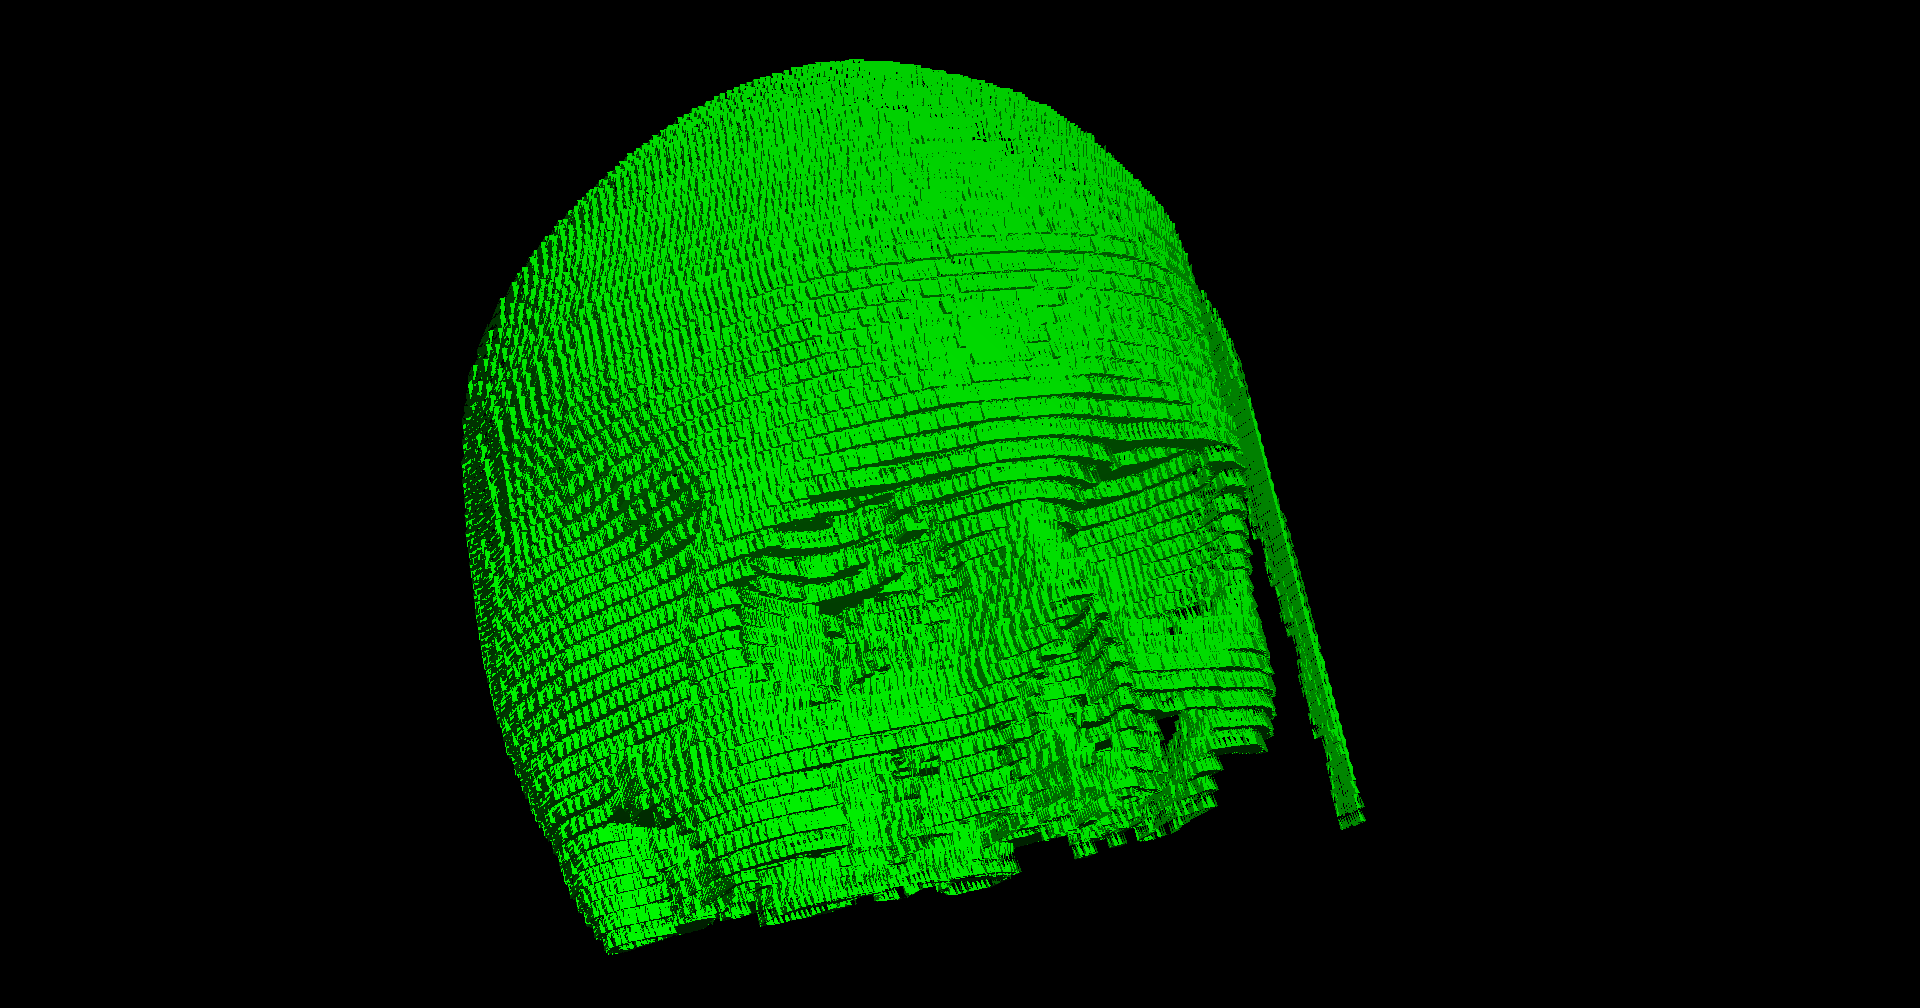
\includegraphics[width=200pt]{manix.png}}
\caption{Manix - seuil de 1250}
\end{figure}

\newpage
\section*{Code source}

\begin{lstlisting}
#include <cstring>
#include <iostream>
#include <vector>
#include <fstream>
#include <stdlib.h> 
#include <algorithm>
#include "math.h"
#include <string>

using namespace std;

class Vector {
public:
  double x;
  double y;
  double z;

  Vector(double x, double y, double z) {
    this->x = x;
    this->y = y;
    this->z = z;
  }

  void add(double x, double y, double z) {
    this->x += x;
    this->y += y;
    this->z += z;
  }

  std::string toString() {
    string s = "";
    s += std::to_string(x) + " ";
    s += std::to_string(y) + " ";
    s += std::to_string(z);
    return s;
  }

};

class Triangle {
public:
  Vector *v1;
  Vector *v2;
  Vector *v3;

  Triangle(Vector* orig, Vector* x, Vector* y, Vector* z) {
    this->v1 = new Vector(orig->x, orig->y, orig->z); v1->add(x->x, x->y, x->z);
    this->v2 = new Vector(orig->x, orig->y, orig->z); v2->add(y->x, y->y, y->z);
    this->v3 = new Vector(orig->x, orig->y, orig->z); v3->add(z->x, z->y, z->z);
  }

  std::string toString() {
    std::string s = "facet normal 0 0 0";

    s += "\nouter loop\n";
    s += "vertex " + v1->toString() + "\n";
    s += "vertex " + v2->toString() + "\n";
    s += "vertex " + v3->toString() + "\n";
    s += "endloop\nendfacet";

    return s;
  }
};

class RawReader {
private:
  std::vector<unsigned short*> data;
  int sizeX;
  int sizeY;
  int sizeZ;
  void load(std::string path);

public:
  unsigned short getValue(int i, int j, int k);
  void seuil(unsigned short s);
  RawReader(std::string path, int sizeX, int sizeY, int sizeZ);
  void marchingCubes(double vWidth, double vHeight, double vDepth, unsigned short treshold);
};

RawReader::RawReader(std::string path, int sizeX, int sizeY, int sizeZ) {
  this->sizeX = sizeX;
  this->sizeY = sizeY;
  this->sizeZ = sizeZ;
  this->load(path);
}

unsigned short RawReader::getValue(int i, int j, int k) {
  return data[k][i * sizeY + j];
}

void RawReader::load(std::string path) {
  std::ifstream f (path.c_str(), ios::in | ios::binary);
  unsigned short c;
  unsigned short *img = new unsigned short [sizeX*sizeY];
  int i = 0;
  while(!f.eof()) {
    f.read((char *)&c,sizeof(short));

    short l = c % 256;
    short r = c / 256;

    img[i++] = l * 256 + r;
    if(i >= sizeX * sizeY) {
      i = 0;
      data.push_back(img);
      img = new unsigned short [sizeX*sizeY];
    }
  }
}

void RawReader::seuil(unsigned short s) {
  for (int i = 0; i < sizeX; ++i) {
    for (int j = 0; j < sizeY; ++j) {
      for (int k = 0; k < sizeZ; ++k) {
        if(getValue(i, j, k) < s) {
          setValue(i, j, k, 0);
        } else {
          setValue(i, j, k, pow(2, 16) - 1);
        }
      }
    }
  }
}

void RawReader::marchingCubes(double vWidth, double vHeight, double vDepth, unsigned short threshold) {
  std::cout << "solid name" << std::endl;
  for (int i = 1; i < sizeX - 1; ++i) {
    for (int j = 1; j < sizeY - 1; ++j) {
      for (int k = 1; k < sizeZ - 1; ++k) {

        if(getValue(i, j, k) > threshold) {

          if(getValue(i + 1, j, k) < threshold) {
            Vector orig((i + 1) * vWidth, j * vHeight, k * vDepth);
            Vector v1(0, 0, vDepth);
            Vector v2(0, vHeight, vDepth);
            Vector v3(0, vHeight, 0);
            Triangle t1(&orig, &v1, &v2, &v3);
            std::cout << t1.toString() << std::endl;
          }

          if(getValue(i - 1, j, k) < threshold) {
            Vector orig((i - 1) * vWidth, j * vHeight, k * vDepth);
            Vector v1(0, 0, vDepth);
            Vector v2(0, vHeight, vDepth);
            Vector v3(0, vHeight, 0);
            Triangle t1(&orig, &v1, &v2, &v3);
            std::cout << t1.toString() << std::endl;
          }

          if(getValue(i, j + 1, k) < threshold) {
            Vector orig(i * vWidth, (j + 1) * vHeight, k * vDepth);
            Vector v1(0, 0, vDepth);
            Vector v2(vWidth, 0, vDepth);
            Vector v3(vWidth, 0, 0);
            Triangle t1(&orig, &v1, &v2, &v3);
            std::cout << t1.toString() << std::endl;
          }
          if(getValue(i, j - 1, k) < threshold) {
            Vector orig(i * vWidth, (j - 1) * vHeight, k * vDepth);
            Vector v1(0, 0, vDepth);
            Vector v2(vWidth, 0, vDepth);
            Vector v3(vWidth, 0, 0);
            Triangle t1(&orig, &v1, &v2, &v3);
            std::cout << t1.toString() << std::endl;
          }
          if(getValue(i, j, k + 1) < threshold) {
            Vector orig(i * vWidth, j * vHeight, (k + 1) * vDepth);
            Vector v1(0, vHeight, 0);
            Vector v2(0, vHeight, 0);
            Vector v3(vWidth, 0, 0);
            Triangle t1(&orig, &v1, &v2, &v3);
            std::cout << t1.toString() << std::endl;
          }
          if(getValue(i, j, k - 1) < threshold) {
            Vector orig(i * vWidth, j * vHeight, (k - 1) * vDepth);
            Vector v1(0, vHeight, 0);
            Vector v2(vWidth, 0, 0);
            Vector v3(vWidth, vHeight, 0);
            Triangle t1(&orig, &v1, &v2, &v3);
            std::cout << t1.toString() << std::endl;
          }
        }
      }
    }
  }
  std::cout << "endsolid name" << std::endl;
}
\end{lstlisting}


\end{document}

